\documentclass[journal]{IEEEtran}

\usepackage[UTF8,scheme=plain,fontset=fandol]{ctex}
\usepackage{amsmath,amssymb,bm}
\usepackage{graphicx}
\usepackage{booktabs}
\usepackage{multirow}
\usepackage{array}
\usepackage{makecell}
\usepackage{stfloats}
\usepackage{enumitem}
\usepackage{url}
\usepackage[hidelinks]{hyperref}

\renewcommand{\abstractname}{摘要}
\renewcommand{\IEEEkeywordsname}{关键词}
\renewcommand{\figurename}{图}
\renewcommand{\tablename}{表}
\renewcommand{\refname}{参考文献}

\newcommand{\qtran}{\textsc{QTran}}
\newcommand{\wm}{\textsc{WM-811K}}
\newcommand{\macroF}{\operatorname{Macro\text{-}F1}}
\newcommand{\bacc}{\operatorname{BAcc}}
\newcommand{\E}{\mathbb{E}}
\newcommand{\R}{\mathbb{R}}
\graphicspath{{figures/}}

\title{QTran-WM：面向类别不平衡晶圆缺陷模式识别的量子自注意力 Transformer}

\author{作者姓名（待补充）%
\thanks{本文为中文初稿，作者、单位、基金和通信信息将在定稿阶段补充。}}

\begin{document}

\maketitle

\begin{abstract}
晶圆图缺陷模式识别是半导体制造缺陷溯源与良率提升的重要环节，但真实产线数据通常同时具有类别极度不平衡、稀有模式样本有限以及测量噪声不可避免等特点。为研究小参数量量子模型在该领域中的适用性，本文提出一种面向晶圆图分类的量子自注意力 Transformer，简称 \qtran。该方法首先以共享的轻量卷积标记器提取晶圆图局部空间特征并形成 $4\times4$ 个特征标记；随后分别使用三个四量子比特参数化量子线路生成查询、键和值，使量子特征映射直接参与不同晶圆区域之间的相关性建模；最后通过双头缩放点积注意力、残差前馈网络和全局平均池化完成九类晶圆模式识别。本文在包含 $172{,}950$ 张有标签晶圆图的 \wm{} 数据集上，将 \qtran{} 与参数量相近的微型 Transformer、MLP-Mixer 和卷积标记混合器进行五随机种子公平比较。主实验中，\qtran{} 仅含 $2{,}345$ 个可训练参数，测试集 Macro-F1 为 $0.602\pm0.053$，高于 MLP-Mixer 和卷积标记混合器，但略低于微型 Transformer 的 $0.607\pm0.027$，配对检验未显示统计显著差异。在更具领域针对性的实验中，\qtran{} 在每类 $25$ 和 $50$ 个训练样本时获得最高的平衡准确率；当晶圆有效区域的缺陷位以 $10\%$ 概率翻转时，其 Macro-F1 保留率达到 $0.772\pm0.049$，为四种模型中最高。实验表明，量子自注意力尚未形成普遍且显著的性能优势，但在受限标注和较强输入扰动条件下呈现出值得进一步验证的潜力。本文工作为量子机器学习从 MNIST、Fashion-MNIST 等通用图像基准走向半导体制造领域提供了可复现的小规模研究范式。
\end{abstract}

\begin{IEEEkeywords}
晶圆图，缺陷模式识别，量子机器学习，量子自注意力，Transformer，类别不平衡，\wm
\end{IEEEkeywords}

\section{引言}

随着集成电路特征尺寸持续缩小和制造工序不断增加，晶圆制造过程对缺陷检测、空间模式识别和根因定位提出了更高要求。晶圆图以二维空间形式记录芯片单元的测试状态；Center、Donut、Edge-Loc、Edge-Ring、Loc、Near-full、Random 和 Scratch 等模式往往与设备状态、工艺漂移或污染机制相关，因此，准确识别晶圆图模式能够为工程人员缩小排查范围，并为制造过程控制和良率改进提供依据\cite{wu2015wafer}。

真实晶圆数据并不满足常规图像分类中近似均衡、独立同分布的理想条件。以公开的 \wm{} 为例，$811{,}457$ 张晶圆图中仅 $172{,}950$ 张具有明确标签；在有标签子集中，正常类 None 占 $85.24\%$，而 Near-full 仅有 $149$ 张，占 $0.086\%$。这意味着一个始终偏向多数类的模型仍可能获得较高的总体准确率，却无法可靠发现最需要关注的稀有缺陷。此外，同一生产批次中的晶圆通常共享工艺背景，若随机按样本划分训练集与测试集，批次信息泄漏会使评估结果过于乐观。因此，面向晶圆图的算法不仅需要处理长尾分布，还应在批次隔离、有限标注和噪声扰动下接受检验。

已有研究主要采用卷积神经网络、残差结构、数据增强和视觉 Transformer 进行晶圆图识别\cite{wang2022residual,yu2023lightweight,fan2024vit}。卷积网络善于捕获局部纹理，却需要逐层扩大感受野才能建立相距较远区域之间的联系；自注意力能够直接建模全局关系，但标准查询、键和值通常由线性投影生成，在本文所关注的极小参数预算下，其表达能力可能受到限制。过采样或强数据增强能够缓解类别不平衡，却可能重复稀有样本并放大噪声。由此产生一个核心问题：能否在不增加模型规模的前提下，引入不同于经典线性映射的特征空间，以改善小样本和扰动条件下的区域关联建模？

参数化量子线路通过数据编码、可训练旋转门和纠缠门构造高维非线性特征映射，已被用于量子分类器和量子核方法\cite{havlicek2019supervised,grant2018hierarchical,schuld2020circuit}。近年来，量子自注意力研究进一步尝试将量子线路用于注意力权重或特征生成\cite{zhao2024qksan,shi2025qsan}。然而，现有量子图像分类工作常集中于 MNIST、Fashion-MNIST 等通用基准。此类数据可以证明算法具备基本分类能力，却不能直接回答量子注意力是否适合类别极不平衡、具有明确空间模式和生产批次结构的晶圆数据。更重要的是，若量子模型拥有更多参数、不同的数据划分或更充分的调参预算，所得优势不能归因于量子机制本身。

基于上述分析，本文建立如下三个研究问题：

\begin{itemize}[leftmargin=1.5em]
  \item \textbf{RQ1：}在共享数据、标记器、分类头、训练流程和近似参数量的条件下，量子查询--键--值映射能否提高晶圆缺陷分类的 Macro-F1 与平衡准确率？
  \item \textbf{RQ2：}当每类仅提供 $25$、$50$、$100$ 或 $200$ 个训练样本时，\qtran{} 是否表现出更好的少样本学习能力？
  \item \textbf{RQ3：}当晶圆有效区域中的缺陷状态受到随机翻转时，\qtran{} 是否能保留更多分类性能？
\end{itemize}

围绕这些问题，本文的主要贡献如下：

\begin{itemize}[leftmargin=1.5em]
  \item 提出面向晶圆图的 \qtran{} 架构。该架构将轻量卷积提取的 $16$ 个区域标记编码到三个独立的四量子比特参数化量子线路中，以量子测量期望值生成查询、键和值，并以双头自注意力建立缺陷区域之间的全局联系。
  \item 建立严格的同规模公平比较方案。四种模型共享输入、卷积标记器、嵌入维度、分类头、损失函数、优化器、训练样本和随机种子，参数量控制在 $2{,}317$--$2{,}359$ 之间；数据按生产批次隔离，并以五个随机种子报告均值、标准差、置信区间和配对检验。
  \item 从标准分类、少样本学习和输入噪声三个层面验证量子自注意力。结果没有支持“量子模型普遍显著优于所有经典模型”的强结论，但显示其在低样本平衡准确率和强噪声性能保留方面具有稳定的探索性优势，为后续电路改进和跨数据集验证提供了实证依据。
\end{itemize}

本文其余内容安排如下：第\ref{sec:preliminaries}节介绍晶圆图、自注意力与参数化量子线路的基础知识；第\ref{sec:method}节给出 \qtran{} 的定义、量子查询--键--值机制和完整工作流程；第\ref{sec:experiment}节说明数据、比较方法、实验设置并分析五随机种子结果；第\ref{sec:conclusion}节总结全文并讨论未来方向。

\section{基础知识}
\label{sec:preliminaries}

\subsection{晶圆图与 \wm{} 数据集}

晶圆图可以表示为二维离散矩阵
\begin{equation}
  \bm{W}\in\{0,1,2\}^{H\times W},
\end{equation}
其中，$0$ 表示晶圆外部或无效位置，$1$ 表示通过测试的有效芯片单元，$2$ 表示未通过测试的缺陷单元。与自然图像不同，晶圆图的类别主要由缺陷单元在晶圆有效区域内的几何分布决定。例如，Edge-Ring 表示缺陷沿晶圆边缘形成环状分布，Scratch 表示缺陷呈细长划痕形态，而 Loc 表示缺陷集中于局部区域。这种数据结构同时包含局部形状与跨区域空间关系。

\wm{} 来源于真实半导体制造流程，是晶圆图缺陷识别中使用广泛的公开基准\cite{wu2015wafer}。原始数据还包含生产批次标识。本文将批次作为分组变量，使同一批次的晶圆只出现在训练、验证或测试中的一个子集，从而降低工艺背景泄漏风险。由于类别极不平衡，本文不把总体准确率作为唯一标准，而将 Macro-F1 与平衡准确率作为主要指标。

\subsection{经典缩放点积自注意力}

给定标记序列
\begin{equation}
  \bm{X}=[\bm{x}_1,\ldots,\bm{x}_N]^\mathsf{T}\in\R^{N\times d},
\end{equation}
经典自注意力首先通过三组线性映射构造查询、键和值：
\begin{equation}
  \bm{Q}=\bm{X}\bm{W}_Q,\quad
  \bm{K}=\bm{X}\bm{W}_K,\quad
  \bm{V}=\bm{X}\bm{W}_V.
  \label{eq:classic_qkv}
\end{equation}
第 $i$ 个标记与第 $j$ 个标记之间的相关性由查询和键的内积给出，缩放点积注意力为\cite{vaswani2017attention}
\begin{equation}
  \operatorname{Attn}(\bm{Q},\bm{K},\bm{V})
  =\operatorname{softmax}\left(
    \frac{\bm{Q}\bm{K}^{\mathsf T}}{\sqrt{d_h}}
  \right)\bm{V},
  \label{eq:attention}
\end{equation}
其中 $d_h$ 为每个注意力头的维度。多头注意力将特征维度划分为若干子空间，使不同注意力头学习不同类型的区域联系。自注意力的关键不在于简单加权，而在于查询和键共同决定数据依赖的权重矩阵，因此查询--键--值映射的特征空间会直接影响相关性估计。

\subsection{量子比特与参数化量子线路}

单量子比特纯态可写为
\begin{equation}
  |\psi\rangle=\alpha|0\rangle+\beta|1\rangle,
  \qquad |\alpha|^2+|\beta|^2=1.
\end{equation}
$n$ 个量子比特的状态属于 $2^n$ 维复向量空间。量子门以酉变换改变状态。本文使用的单比特旋转门为
\begin{align}
  R_y(\theta)&=
  \begin{bmatrix}
    \cos(\theta/2)&-\sin(\theta/2)\\
    \sin(\theta/2)& \cos(\theta/2)
  \end{bmatrix},\\
  R_z(\theta)&=
  \begin{bmatrix}
    e^{-i\theta/2}&0\\
    0&e^{i\theta/2}
  \end{bmatrix}.
\end{align}
受控非门 CNOT 根据控制比特状态翻转目标比特，可在多量子比特之间建立纠缠关系。参数化量子线路将经典输入 $\bm{x}$ 编码为量子态，再通过带参数的酉变换 $U(\bm{x},\bm{\theta})$ 处理，最终测量可观测量 $O$：
\begin{equation}
  f(\bm{x};\bm{\theta})=
  \langle0|U^{\dagger}(\bm{x},\bm{\theta})
  O,U(\bm{x},\bm{\theta})|0\rangle.
  \label{eq:pqc}
\end{equation}
由于量子态演化包含周期旋转、纠缠和测量，式\eqref{eq:pqc}定义了不同于单层经典线性投影的非线性映射。本文在 GPU 上以状态向量模拟量子线路，并通过自动微分与经典网络联合优化；该设置不需要真实量子硬件，但模拟开销随量子比特数指数增长，因此电路被限制为四量子比特。

\subsection{量子特征映射与自注意力的联系}

经典自注意力使用式\eqref{eq:classic_qkv}中的线性变换决定标记间相似度。若以量子特征映射 $\phi_{\bm{\theta}}(\cdot)$ 替换这些线性变换，则相关性变为
\begin{equation}
  s_{ij}=
  \frac{
    \phi_{\bm{\theta}_Q}(\bm{x}_i)^{\mathsf T}
    \phi_{\bm{\theta}_K}(\bm{x}_j)
  }{\sqrt{d_h}}.
  \label{eq:quantum_similarity}
\end{equation}
此时，量子线路不直接替代 softmax，也不改变注意力的基本语义，而是改变查询和键所在的特征空间；量子值映射则改变被聚合的信息表示。

\textbf{强调：}本文并不把希尔伯特空间维度本身等同于可验证的“量子优势”。在四量子比特 GPU 模拟条件下，合理且可检验的命题是：量子映射所引入的归纳偏置是否能在相同参数预算和相同训练信息下改善晶圆区域关联。该命题必须由配对、多随机种子实验验证，而不能由理论维度直接推出。

\section{面向晶圆缺陷识别的量子自注意力 Transformer}
\label{sec:method}

\subsection{问题定义}

给定带标签晶圆数据集
\begin{equation}
  \mathcal{D}=\{(\bm{W}_i,y_i,g_i)\}_{i=1}^{M},
\end{equation}
其中 $\bm{W}_i$ 为晶圆图，$y_i\in\{1,\ldots,9\}$ 为模式标签，$g_i$ 为生产批次。目标是在保证训练、验证和测试批次集合两两不相交的条件下，学习分类函数 $F_{\bm{\Theta}}(\bm{W})$。本文将 \qtran{} 定义如下。

\textbf{定义 1（量子自注意力晶圆分类器）：}若模型以共享卷积网络生成区域标记，以彼此独立的参数化量子线路生成 $\bm{Q}$、$\bm{K}$ 和 $\bm{V}$，并通过经典缩放点积注意力聚合量子测量特征，则称该混合量子--经典网络为量子自注意力晶圆分类器。

\subsection{总体架构}

\begin{figure*}[t]
  \centering
  \fbox{\parbox[c][4.2cm][c]{0.94\textwidth}{\centering
  \textbf{QTran-WM 总体框架图占位}\par\vspace{0.5em}
  待绘制内容：$32\times32$ 晶圆图 $\rightarrow$ 有效区域/缺陷双通道 $\rightarrow$ 轻量卷积标记器 $\rightarrow$ $16\times4$ 标记序列 $\rightarrow$ 三个独立四量子比特 Q/K/V 电路 $\rightarrow$ 双头量子自注意力 $\rightarrow$ 残差前馈网络 $\rightarrow$ 九类输出。}}
  \caption{所提出 QTran-WM 的总体架构。正式框架图将在定稿阶段绘制；当前占位文字给出必须包含的模块和数据流。}
  \label{fig:framework}
\end{figure*}

如图\ref{fig:framework}所示，\qtran{} 由输入编码、共享卷积标记器、量子查询--键--值映射、经典多头注意力以及分类头五部分组成。量子线路只承担查询、键和值的生成，其余部分保留为经典可微模块。这一边界既使量子机制具有明确归因，又避免对前馈层进行不必要的状态向量模拟。

\subsection{晶圆双通道编码与特征标记化}

首先将晶圆图转换为两个二值通道：
\begin{align}
  \bm{X}^{(e)}_{u,v}&=\mathbb{I}[\bm{W}_{u,v}>0],\\
  \bm{X}^{(d)}_{u,v}&=\mathbb{I}[\bm{W}_{u,v}=2],
\end{align}
其中 $\bm{X}^{(e)}$ 描述晶圆有效区域，$\bm{X}^{(d)}$ 描述缺陷位置。双通道编码使网络能够区分“晶圆外部”与“晶圆内部的正常单元”，避免将二者同时视为无缺陷背景。原始晶圆图采用最近邻插值缩放至 $32\times32$，以保持离散状态码。

共享标记器依次包含 $2\rightarrow12$ 的 $3\times3$ 卷积、组归一化、GELU、$12\rightarrow16$ 的步长为 2 的 $3\times3$ 卷积、组归一化、GELU、自适应 $4\times4$ 池化以及 $16\rightarrow4$ 的 $1\times1$ 投影。输出展平为
\begin{equation}
  \bm{T}=\operatorname{Flatten}(f_{\mathrm{CNN}}(\bm{X}))
  +\bm{P}\in\R^{16\times4},
  \label{eq:tokens}
\end{equation}
其中 $\bm{P}$ 是可学习位置嵌入。$16$ 个标记分别代表晶圆的不同空间区域，四维嵌入与四量子比特输入一一对应。

\subsection{四量子比特查询--键--值映射}

对于任一标记 $\bm{t}_i=[t_{i,1},\ldots,t_{i,4}]$，先将其压缩为有界旋转角
\begin{equation}
  \phi_{i,j}=\pi\tanh(t_{i,j}),\qquad j=1,\ldots,4.
  \label{eq:angle_encoding}
\end{equation}
该处理避免未经约束的卷积特征产生过大的周期性角度变化。随后通过 $R_y(\phi_{i,j})$ 将四个分量分别编码至四个量子比特。每个变分层由一组可训练 $R_y$、一组可训练 $R_z$ 和环形 CNOT 组成。深度 $L=2$ 时，量子线路可写为
\begin{equation}
  U_{\bm{\theta}}(\bm{t}_i)
  =\prod_{l=1}^{2}
  \left[
    U_{\mathrm{ring}}
    \prod_{j=1}^{4}R_z(\theta^{z}_{l,j})R_y(\theta^{y}_{l,j})
  \right]
  \prod_{j=1}^{4}R_y(\phi_{i,j}).
  \label{eq:q_circuit}
\end{equation}
其中，$U_{\mathrm{ring}}$ 按 $1\rightarrow2\rightarrow3\rightarrow4\rightarrow1$ 的方向施加 CNOT，以建立四个区域特征分量之间的纠缠。所有可训练旋转角从 $[-0.1,0.1]$ 均匀初始化，使浅层线路从接近恒等映射的区域开始训练，同时保持查询、键和值三条分支的非对称性。

在线路末端测量每个量子比特的 Pauli-$Z$ 期望值：
\begin{equation}
  \phi_{\bm{\theta}}(\bm{t}_i)=
  [\langle Z_1\rangle,\ldots,\langle Z_4\rangle]\in[-1,1]^4.
  \label{eq:z_measurement}
\end{equation}
三个结构相同但参数独立的量子线路分别得到
\begin{equation}
  \bm{q}_i=\phi_{\bm{\theta}_Q}(\bm{t}_i),\quad
  \bm{k}_i=\phi_{\bm{\theta}_K}(\bm{t}_i),\quad
  \bm{v}_i=\phi_{\bm{\theta}_V}(\bm{t}_i).
  \label{eq:quantum_qkv}
\end{equation}
独立参数保证三条分支可分别学习“检索需求”“匹配索引”和“待聚合内容”，而不是重复使用同一个量子表示。

\subsection{双头注意力与分类头}

将四维量子输出划分为 $H=2$ 个注意力头，每个头维度 $d_h=2$。第 $h$ 个头的注意力为
\begin{equation}
  \bm{A}^{(h)}=
  \operatorname{softmax}\left(
    \frac{\bm{Q}^{(h)}(\bm{K}^{(h)})^{\mathsf T}}{\sqrt{2}}
  \right),\quad
  \bm{C}^{(h)}=\bm{A}^{(h)}\bm{V}^{(h)}.
\end{equation}
两个头拼接后经过 $4\rightarrow4$ 线性输出层，并与输入形成残差连接。随后使用层归一化和 $4\rightarrow8\rightarrow4$ 的前馈网络：
\begin{align}
  \bm{T}'&=\operatorname{LN}\bigl(\bm{T}+\operatorname{Dropout}(\bm{C}\bm{W}_O)\bigr),\\
  \bm{T}''&=\operatorname{LN}\bigl(\bm{T}'+
  \operatorname{Dropout}(\operatorname{FFN}(\bm{T}'))\bigr).
\end{align}
最后对 $16$ 个标记求均值，并以层归一化和 $4\rightarrow9$ 线性层输出类别概率：
\begin{equation}
  \hat{\bm{y}}=\operatorname{softmax}\left(
  \bm{W}_c\operatorname{LN}\left(
  \frac{1}{16}\sum_{i=1}^{16}\bm{T}''_i
  \right)+\bm{b}_c\right).
\end{equation}

\subsection{训练目标与完整工作流程}

为降低过度自信，本文使用标签平滑系数 $\varepsilon=0.05$ 的交叉熵损失。类别采样概率采用平方根逆频率校正，类别 $c$ 中样本的权重为
\begin{equation}
  w_c=n_c^{-\gamma},\qquad \gamma=0.5,
\end{equation}
它位于自然采样（$\gamma=0$）和完全逆频率平衡（$\gamma=1$）之间，既提高稀有类被抽取的概率，又避免多数类在训练中几乎消失。

完整工作流程如下。

\begin{enumerate}[leftmargin=1.8em]
  \item \textbf{批次隔离：}按照生产批次 $g_i$ 将全部有标签数据划分为训练、验证和测试集。
  \item \textbf{离散预处理：}将晶圆图以最近邻方式缩放至 $32\times32$，构造有效区域和缺陷双通道。
  \item \textbf{数据增强：}仅对训练样本随机实施 $0^\circ$、$90^\circ$、$180^\circ$、$270^\circ$ 旋转及水平、垂直翻转。
  \item \textbf{标记生成：}共享轻量卷积标记器将输入转换为 $16$ 个四维区域标记。
  \item \textbf{量子映射：}根据式\eqref{eq:angle_encoding}--\eqref{eq:quantum_qkv}并行生成量子查询、键和值。
  \item \textbf{关系聚合：}双头缩放点积注意力建立所有晶圆区域之间的联系，并由残差前馈网络更新标记。
  \item \textbf{联合优化：}使用 AdamW 和余弦学习率调度器端到端优化经典参数与量子门参数，以验证集 Macro-F1 选择最佳检查点。
\end{enumerate}

\subsection{参数规模与可实现性}

\qtran{} 的总可训练参数量为 $2{,}345$。三个量子投影各包含两层可训练 $R_y$ 与 $R_z$ 旋转，共有 $3\times2\times4\times2=48$ 个量子门参数；其余参数来自共享卷积标记器、位置嵌入、经典注意力输出、前馈层和分类头。四量子比特状态向量仅有 $2^4=16$ 个复振幅，因此可在单张 GPU 上进行批量模拟。该设计用于验证量子特征映射的学习效果，并不声称获得硬件级加速；从本文实测训练时间看，量子模拟仍明显慢于经典模型。

\section{实验与结果分析}
\label{sec:experiment}

为回答第\ref{sec:method}节之前提出的三个研究问题，实验分为四个部分：

\begin{itemize}[leftmargin=1.5em]
  \item \textbf{数据与公平性审计：}检查类别分布、批次隔离、可训练参数量和梯度完整性；
  \item \textbf{主分类实验：}在相同训练与测试数据上比较四种同规模模型，并进行五随机种子配对统计；
  \item \textbf{少样本实验：}在每类 $25$、$50$、$100$ 和 $200$ 个训练样本下检验有限标注能力；
  \item \textbf{输入噪声实验：}在不重新训练的情况下逐步提高缺陷位翻转概率，分析性能保留率。
\end{itemize}

\subsection{数据集与类别分布}

本文使用 \wm{} 有标签子集，共包含 $172{,}950$ 张晶圆图和 $10{,}762$ 个生产批次。九类样本分布见表\ref{tab:class_distribution}和图\ref{fig:class_distribution}。None 类占比为 $85.245\%$，Near-full 类仅占 $0.086\%$，最大类与最小类样本数之比接近 $990:1$。这一分布说明，若仅报告总体准确率，将严重掩盖稀有类识别错误。

\begin{table}[t]
  \centering
  \caption{\wm{} 有标签子集的类别分布}
  \label{tab:class_distribution}
  \resizebox{\columnwidth}{!}{%
  \begin{tabular}{lrr@{\quad}lrr}
    \toprule
    类别 & 数量 & 占比(\%) & 类别 & 数量 & 占比(\%)\\
    \midrule
    Center    & 4,294   & 2.483 & Donut     & 555     & 0.321\\
    Edge-Loc  & 5,189   & 3.000 & Edge-Ring & 9,680   & 5.597\\
    Loc       & 3,593   & 2.078 & Near-full & 149     & 0.086\\
    Random    & 866     & 0.501 & Scratch   & 1,193   & 0.690\\
    None      & 147,431 & 85.245& 合计      & 172,950 & 100.000\\
    \bottomrule
  \end{tabular}}
\end{table}

\begin{figure}[t]
  \centering
  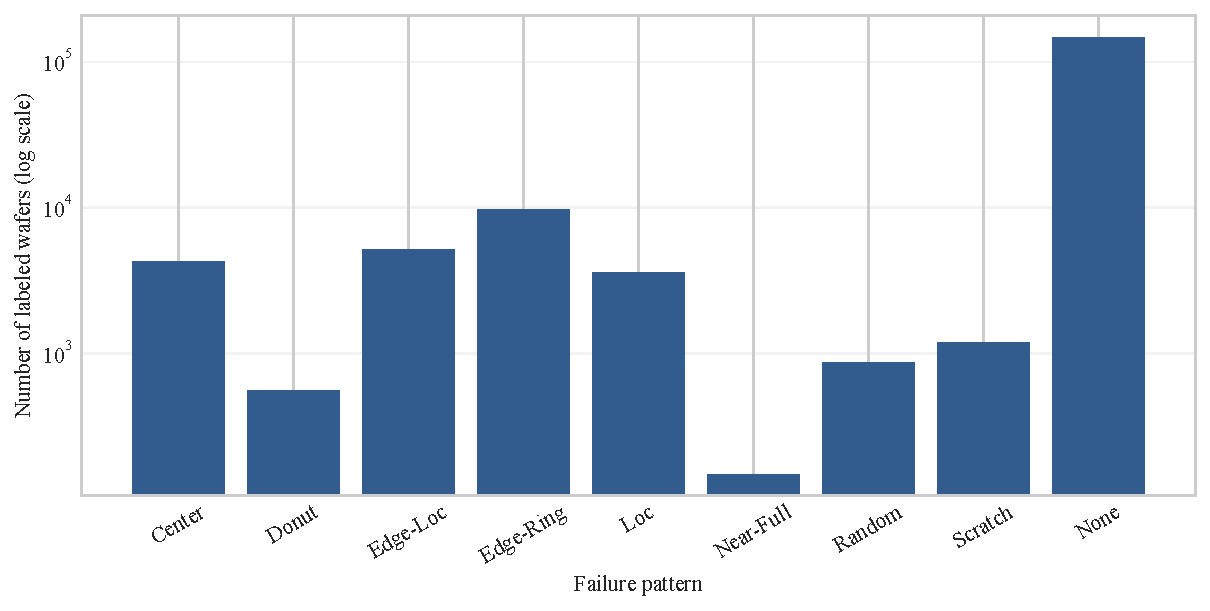
\includegraphics[width=\columnwidth]{class_distribution.pdf}
  \caption{\wm{} 有标签子集的类别分布。纵轴采用对数刻度，以同时显示多数类与稀有类。}
  \label{fig:class_distribution}
\end{figure}

按照固定划分种子 $20260815$ 进行生产批次互斥划分后，完整训练、验证和测试集分别包含 $121{,}072$、$25{,}943$ 和 $25{,}935$ 个样本。主实验为了控制计算预算，对训练集中每类最多使用 $2{,}000$ 个样本，实际训练样本数为 $11{,}968$；验证集与测试集不截断，保留自然类别分布和全部稀有样本。需要指出，训练截断属于本文小参数量可行性实验的设计选择，不代表对完整 \wm{} 训练上限的估计。

\subsection{比较模型与公平性约束}

本文选择三种结构互补的经典模型作为比较对象。

\begin{itemize}[leftmargin=1.5em]
  \item \textbf{Tiny Transformer：}使用 PyTorch 多头自注意力，以经典线性层生成查询、键和值；
  \item \textbf{MLP-Mixer：}使用 $16\rightarrow2\rightarrow16$ 的标记 MLP 和 $4\rightarrow8\rightarrow4$ 的通道 MLP 混合信息；
  \item \textbf{CNN Token Mixer：}使用深度可分离 $3\times3$ 卷积进行局部标记混合，并使用 $4\rightarrow8\rightarrow4$ 通道 MLP。
\end{itemize}

四种模型共享完全相同的双通道输入、卷积标记器、位置嵌入、四维标记、分类头、数据增强、采样器、优化器、训练轮数上限、早停规则和随机种子。参数量见表\ref{tab:param_fairness}。相对于 \qtran{}，三种基线的绝对参数差分别为 $12$、$14$ 和 $28$，最大相对差仅 $1.19\%$，满足本文预先设定的 $5\%$ 参数容差。

\begin{table}[t]
  \centering
  \caption{模型参数量公平性审计}
  \label{tab:param_fairness}
  \begin{tabular}{lrr}
    \toprule
    模型 & 参数量 & 相对 \qtran{} 差异(\%)\\
    \midrule
    \qtran{} & 2,345 & 0.00\\
    Tiny Transformer & 2,357 & 0.51\\
    MLP-Mixer & 2,359 & 0.60\\
    CNN Token Mixer & 2,317 & $-1.19$\\
    \bottomrule
  \end{tabular}
\end{table}

\subsection{实现细节与评价指标}

实验在 NVIDIA GeForce RTX 4090 GPU 上运行，经典部分使用 PyTorch，量子线路使用 DeepQuantum 的可微四量子比特状态向量模拟器\cite{paszke2019pytorch,he2025deepquantum}，绘图使用 Matplotlib。主要超参数见表\ref{tab:settings}。每个模型分别使用随机种子 $42$、$52$、$62$、$72$ 和 $82$ 训练。验证集只用于选择最佳轮次，测试集仅在最佳检查点确定后评估一次。

\begin{table}[t]
  \centering
  \caption{主实验设置}
  \label{tab:settings}
  \resizebox{\columnwidth}{!}{%
  \begin{tabular}{ll@{\quad}ll}
    \toprule
    项目 & 设置 & 项目 & 设置\\
    \midrule
    输入尺寸 & $32\times32\times2$ & 标记数 & 16\\
    标记维度 & 4 & 注意力头数 & 2\\
    量子比特数 & 4 & 电路深度 & 2\\
    Batch size & 64 & 最大轮数 & 60\\
    初始学习率 & $5\times10^{-4}$ & 权重衰减 & $3\times10^{-2}$\\
    Dropout & 0.15 & 标签平滑 & 0.05\\
    梯度裁剪 & 1.0 & 早停耐心值 & 12\\
    采样幂指数 & 0.5 & 训练类上限 & 2,000\\
    \bottomrule
  \end{tabular}}
\end{table}

对每一类别 $c$，精确率、召回率和 F1 分别记为 $P_c$、$R_c$ 和 $F1_c$。主要指标定义为
\begin{align}
  \macroF&=\frac{1}{C}\sum_{c=1}^{C}
  \frac{2P_cR_c}{P_c+R_c},\\
  \bacc&=\frac{1}{C}\sum_{c=1}^{C}R_c,
\end{align}
其中 $C=9$。Macro-F1 同时惩罚精确率或召回率偏低的类别，平衡准确率等价于各类召回率的宏平均。对于每一对模型，本文先在相同随机种子上计算指标差，再报告差值均值、$95\%$ 置信区间、胜率和双侧配对 $t$ 检验 $p$ 值。由于仅有五个随机种子，统计功效有限，$p\ge0.05$ 的趋势不表述为显著优势。

\subsection{主分类结果}

表\ref{tab:main_results}给出五随机种子测试结果，图\ref{fig:main_f1}和图\ref{fig:main_bacc}分别显示 Macro-F1 与平衡准确率。可以得到以下结论。

\begin{itemize}[leftmargin=1.5em]
  \item \textbf{Macro-F1：}\qtran{} 达到 $0.602\pm0.053$，高于 MLP-Mixer 的 $0.582\pm0.071$ 和 CNN Token Mixer 的 $0.596\pm0.045$，但低于 Tiny Transformer 的 $0.607\pm0.027$。因此，RQ1 的强命题“量子模型普遍优于所有同规模经典模型”未得到支持。
  \item \textbf{平衡准确率：}\qtran{} 的结果为 $0.648\pm0.069$，低于三种经典模型。其 Macro-F1 排名高于平衡准确率排名，说明该模型在部分稀有类上取得了较均衡的精确率--召回率折中，但平均召回率仍有提升空间。
  \item \textbf{总体准确率：}MLP-Mixer 以 $0.889\pm0.007$ 最高，\qtran{} 为 $0.874\pm0.029$。考虑到 None 类占比超过 $85\%$，这一指标主要作为补充，不用于判定长尾识别优势。
  \item \textbf{稳定性：}\qtran{} 的 Macro-F1 标准差大于 Tiny Transformer 和 CNN Token Mixer，表明参数化量子线路仍存在明显的种子敏感性。窄范围量子参数初始化缓解了训练失败，但尚未完全解决优化方差。
\end{itemize}

\begin{table*}[t]
  \centering
  \caption{五随机种子主实验结果（均值$\pm$标准差）}
  \label{tab:main_results}
  \begin{tabular}{lrrrrrr}
    \toprule
    模型 & 参数量 & Accuracy & Macro-Precision & Balanced Accuracy & Macro-F1 & 训练时间(s)\\
    \midrule
    \qtran{} & 2,345 & $0.874\pm0.029$ & $0.587\pm0.048$ & $0.648\pm0.069$ & $0.602\pm0.053$ & $367.538\pm108.783$\\
    Tiny Transformer & 2,357 & $0.863\pm0.038$ & $0.581\pm0.035$ & $0.683\pm0.043$ & $0.607\pm0.027$ & $96.769\pm9.367$\\
    MLP-Mixer & 2,359 & $0.889\pm0.007$ & $0.544\pm0.066$ & $0.652\pm0.073$ & $0.582\pm0.071$ & $99.857\pm33.056$\\
    CNN Token Mixer & 2,317 & $0.884\pm0.023$ & $0.567\pm0.028$ & $0.666\pm0.059$ & $0.596\pm0.045$ & $96.710\pm30.940$\\
    \bottomrule
  \end{tabular}
\end{table*}

\begin{figure}[t]
  \centering
  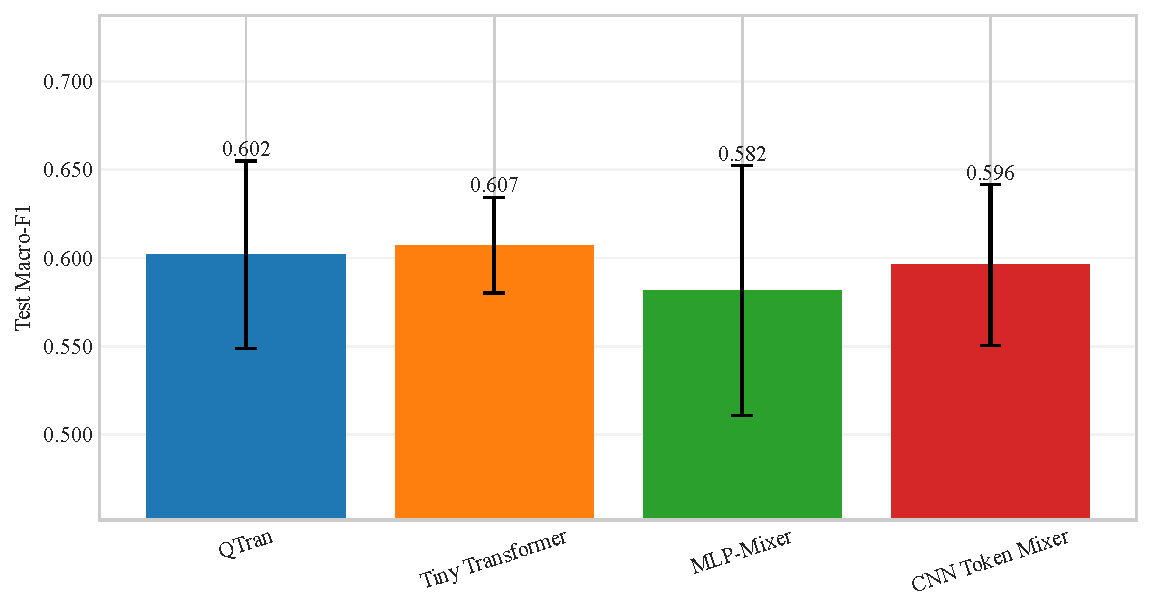
\includegraphics[width=\columnwidth]{main_macro_f1.pdf}
  \caption{五随机种子主实验 Macro-F1。误差棒表示标准差。}
  \label{fig:main_f1}
\end{figure}

\begin{figure}[t]
  \centering
  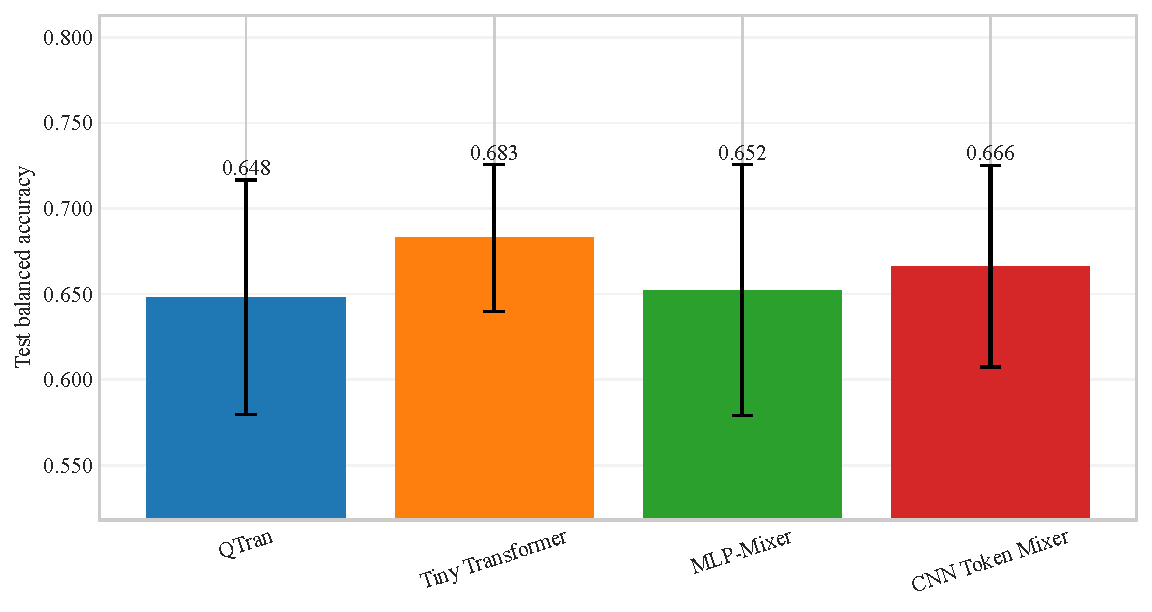
\includegraphics[width=\columnwidth]{main_balanced_accuracy.pdf}
  \caption{五随机种子主实验平衡准确率。误差棒表示标准差。}
  \label{fig:main_bacc}
\end{figure}

表\ref{tab:paired_main}进一步给出以 \qtran{} 为参考的 Macro-F1 配对检验。\qtran{} 相对 MLP-Mixer 和 CNN Token Mixer 的平均差为正，相对 Tiny Transformer 的差为负；所有置信区间均跨越零，且 $p$ 值均大于 $0.05$。因此，当前证据只能说明四种约 $2.3$k 参数模型处于相近性能区间，不能声称 \qtran{} 已取得统计显著的整体领先。

\begin{table}[t]
  \centering
  \caption{主实验 Macro-F1 配对统计（\qtran{} 减比较模型）}
  \label{tab:paired_main}
  \resizebox{\columnwidth}{!}{%
  \begin{tabular}{lrrrr}
    \toprule
    比较模型 & 平均差 & 95\% CI & 胜率 & $p$ 值\\
    \midrule
    Tiny Transformer & $-0.006$ & $[-0.045,0.034]$ & 0.600 & 0.714\\
    MLP-Mixer & $+0.020$ & $[-0.100,0.140]$ & 0.600 & 0.667\\
    CNN Token Mixer & $+0.006$ & $[-0.100,0.111]$ & 0.600 & 0.889\\
    \bottomrule
  \end{tabular}}
\end{table}

\subsection{少样本学习分析}

为回答 RQ2，本文保持验证集、测试集和所有模型超参数不变，仅将训练数据限制为每类 $K\in\{25,50,100,200\}$ 个样本。每个 $K$ 值仍使用五个相同随机种子，因而比较同时控制了样本选择和参数初始化。结果见表\ref{tab:fewshot}和图\ref{fig:fewshot}。

\begin{table*}[t]
  \centering
  \caption{不同每类样本数下的少样本结果（均值$\pm$标准差）}
  \label{tab:fewshot}
  \begin{tabular}{crrrrrrrr}
    \toprule
    & \multicolumn{2}{c}{\qtran{}} & \multicolumn{2}{c}{Tiny Transformer} & \multicolumn{2}{c}{MLP-Mixer} & \multicolumn{2}{c}{CNN Token Mixer}\\
    \cmidrule(lr){2-3}\cmidrule(lr){4-5}\cmidrule(lr){6-7}\cmidrule(lr){8-9}
    $K$ & Macro-F1 & BAcc & Macro-F1 & BAcc & Macro-F1 & BAcc & Macro-F1 & BAcc\\
    \midrule
    25  & $.121\pm.072$ & $.253\pm.058$ & $.128\pm.086$ & $.227\pm.089$ & $.122\pm.061$ & $.232\pm.026$ & $.095\pm.033$ & $.150\pm.044$\\
    50  & $.176\pm.056$ & $.333\pm.054$ & $.140\pm.129$ & $.272\pm.146$ & $.201\pm.126$ & $.289\pm.103$ & $.138\pm.047$ & $.222\pm.075$\\
    100 & $.225\pm.076$ & $.398\pm.089$ & $.196\pm.162$ & $.353\pm.151$ & $.270\pm.076$ & $.413\pm.044$ & $.220\pm.090$ & $.302\pm.138$\\
    200 & $.328\pm.024$ & $.484\pm.030$ & $.329\pm.112$ & $.493\pm.070$ & $.311\pm.077$ & $.459\pm.057$ & $.354\pm.075$ & $.509\pm.075$\\
    \bottomrule
  \end{tabular}
\end{table*}

\begin{figure}[t]
  \centering
  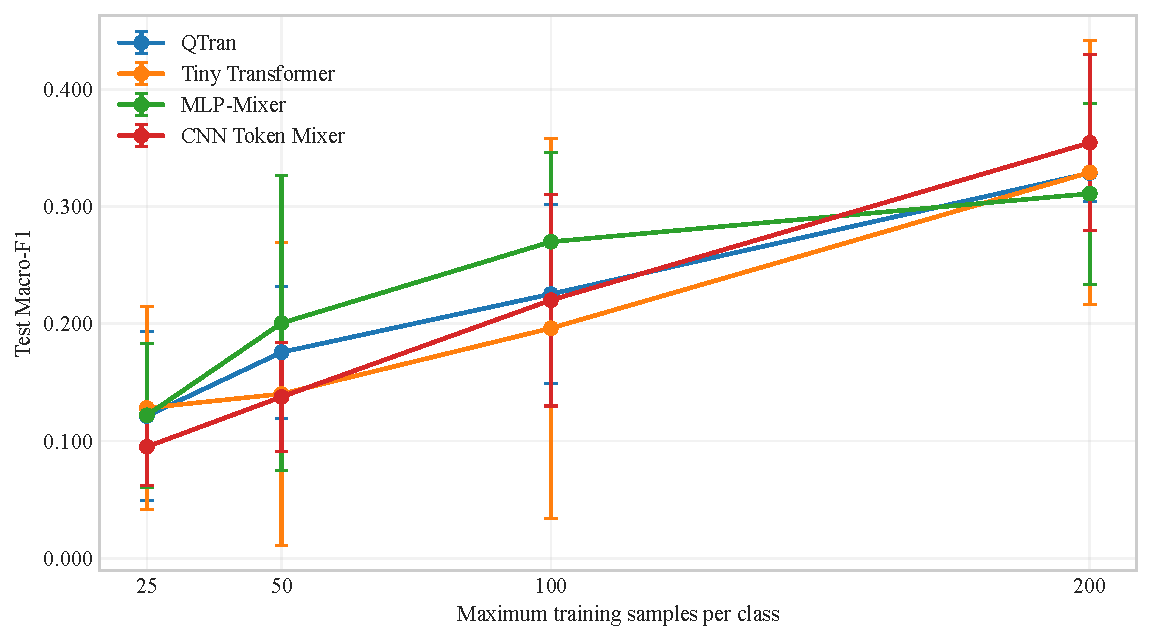
\includegraphics[width=\columnwidth]{few_shot_macro_f1.pdf}
  \caption{不同每类训练样本数下的 Macro-F1。阴影或误差棒表示五种子标准差。}
  \label{fig:fewshot}
\end{figure}

少样本实验呈现出三方面特征。

\begin{itemize}[leftmargin=1.5em]
  \item 当 $K=25$ 和 $K=50$ 时，\qtran{} 分别取得 $0.253$ 和 $0.333$ 的最高平衡准确率，说明量子查询--键--值映射在极少标签条件下更倾向于覆盖多种类别，而非只拟合多数或容易类别。
  \item 从四个 $K$ 值平均的 Macro-F1 看，\qtran{} 为 $0.213$，高于 Tiny Transformer 的 $0.198$ 和 CNN Token Mixer 的 $0.202$，低于 MLP-Mixer 的 $0.226$。以每个 $(K,\text{seed})$ 配对后，\qtran{} 相对 Tiny Transformer 和 CNN Token Mixer 的平均差分别为 $+0.014$ 和 $+0.011$，相对 MLP-Mixer 为 $-0.013$；三项 $p$ 值分别为 $0.746$、$0.422$ 和 $0.783$。
  \item 随 $K$ 增大，各模型整体性能上升，但单一模型并未在所有样本规模上占优。因此，RQ2 得到的是局部而非普遍支持：\qtran{} 的优势主要出现在最受限的类别覆盖指标上，尚不能表述为显著的少样本优势。
\end{itemize}

\subsection{输入噪声鲁棒性分析}

为回答 RQ3，本文对每个已训练最佳检查点直接进行测试，不使用噪声样本继续训练。对于晶圆有效区域中的每个位置，以概率 $\eta$ 翻转缺陷通道：
\begin{equation}
  \widetilde{X}^{(d)}_{u,v}=
  \begin{cases}
  1-X^{(d)}_{u,v}, & r_{u,v}<\eta\ \text{且}\ X^{(e)}_{u,v}=1,\\
  X^{(d)}_{u,v}, & \text{其他情况},
  \end{cases}
\end{equation}
其中 $r_{u,v}\sim\mathcal{U}(0,1)$，同一样本在不同模型间使用相同噪声种子。噪声水平为 $0$、$1\%$、$3\%$、$5\%$ 和 $10\%$。定义 Macro-F1 保留率
\begin{equation}
  \rho(\eta)=\frac{\macroF(\eta)}{\macroF(0)}.
\end{equation}

图\ref{fig:noise}显示，低噪声区间四种模型下降接近；当噪声增至 $5\%$ 时，\qtran{} 的 Macro-F1 为 $0.559\pm0.057$，略高于其余模型；在 $10\%$ 噪声下，\qtran{} 达到 $0.466\pm0.065$，保留率为 $0.772\pm0.049$，均为四种模型中最高。相比之下，Tiny Transformer 的保留率为 $0.729\pm0.023$，MLP-Mixer 为 $0.763\pm0.061$，CNN Token Mixer 为 $0.737\pm0.007$。

\begin{figure}[t]
  \centering
  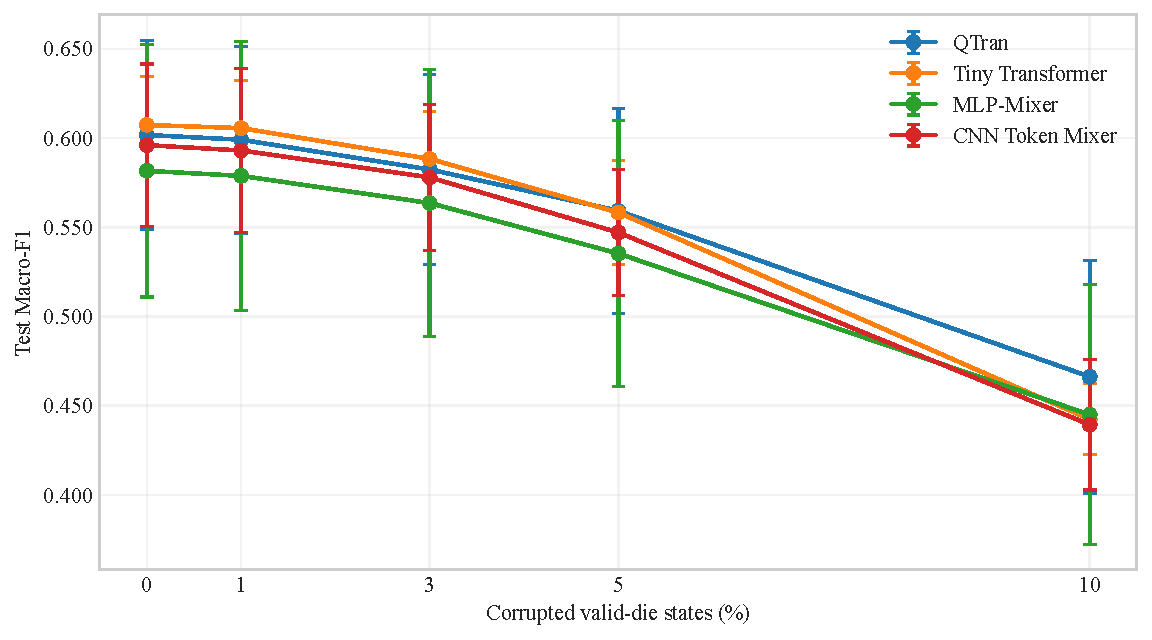
\includegraphics[width=\columnwidth]{noise_robustness_macro_f1.pdf}
  \caption{不同缺陷位翻转概率下的测试集 Macro-F1。模型不使用噪声数据重新训练。}
  \label{fig:noise}
\end{figure}

配对检验中，\qtran{} 在 $10\%$ 噪声下的保留率相对 Tiny Transformer、MLP-Mixer 和 CNN Token Mixer 分别提高 $0.043$、$0.009$ 和 $0.035$，对应胜率为 $0.600$、$0.400$ 和 $0.800$；$95\%$ 置信区间均跨越零，$p$ 值分别为 $0.213$、$0.444$ 和 $0.167$。因此，强噪声下的领先是一项一致方向较好的探索性结果，但尚未达到统计显著。可能的解释是：$\tanh$ 角度压缩、量子测量的有界输出以及跨量子比特纠缠共同限制了局部输入翻转对查询--键相似度的影响。该解释仍需通过去除角度压缩、去除纠缠和匹配有界激活的经典对照实验分别验证。

\subsection{计算代价分析}

图\ref{fig:time}给出平均训练时间。\qtran{} 的平均训练时间为 $367.54$ 秒，约为三种经典模型的 $3.7$--$3.8$ 倍。虽然四量子比特电路本身很小，但每个批次需要对 $16$ 个标记的三条 Q/K/V 分支进行状态向量模拟和反向传播，因而参数少不等同于模拟速度快。

\begin{figure}[t]
  \centering
  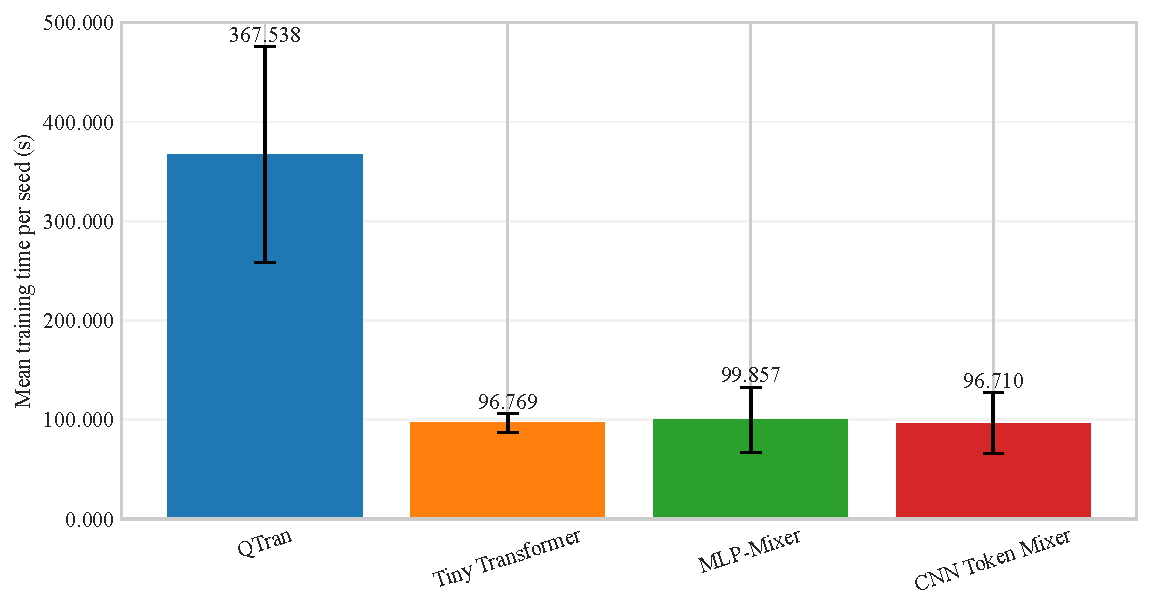
\includegraphics[width=\columnwidth]{training_time.pdf}
  \caption{五随机种子的平均训练时间。误差棒表示标准差。}
  \label{fig:time}
\end{figure}

本文不把训练速度作为 \qtran{} 的优势，也不根据 GPU 模拟结果推断真实量子硬件的时延或能耗。现阶段该模型的价值在于以可控规模验证量子自注意力的归纳偏置。若未来部署到真实硬件，还需考虑数据加载、测量次数、门误差、量子--经典通信和批处理能力。

\subsection{综合讨论}

结合三组实验，可以对研究问题作出以下回答。

\begin{itemize}[leftmargin=1.5em]
  \item 对于 RQ1，\qtran{} 在相同参数预算下与三种经典模型处于同一性能区间，Macro-F1 高于两种基线但未超过 Tiny Transformer，且差异不显著。量子 Q/K/V 是可训练且有效的替代映射，但当前结果不足以证明一般性量子优势。
  \item 对于 RQ2，\qtran{} 在每类 $25$ 和 $50$ 个样本时获得最佳平衡准确率，在跨样本规模平均 Macro-F1 上位居第二。结果支持“极少标签时改善类别覆盖”的弱假设，但不支持“所有少样本规模均最优”的强假设。
  \item 对于 RQ3，\qtran{} 在 $5\%$ 和 $10\%$ 噪声下取得最高 Macro-F1，并在 $10\%$ 噪声下取得最高保留率。该趋势与本文的鲁棒性动机一致，但五种子检验尚未显著，应增加随机种子和噪声类型验证。
\end{itemize}

本文仍存在四点限制。第一，所有量子线路均由 GPU 状态向量模拟，未包含真实量子设备的采样噪声和门噪声。第二，实验只使用一个晶圆公开数据集，无法直接推断至其他工厂、工艺节点或复合缺陷。第三，五个随机种子使置信区间较宽，尤其是量子模型的种子方差仍然较大。第四，本文为了可行性将主训练集限制为每类最多 $2{,}000$ 张，尚未比较完整训练集上的性能上限。后续结论应优先通过增加种子、完整数据训练、量子电路消融和跨数据集验证强化，而不是更换较弱基线或仅报告有利随机种子。

\section{总结与展望}
\label{sec:conclusion}

本文针对 \wm{} 晶圆图类别极不平衡、稀有模式样本有限和输入状态可能受扰动的问题，提出了面向半导体制造领域的量子自注意力 Transformer。该方法以轻量卷积网络提取 $16$ 个四维区域标记，利用三个独立的四量子比特参数化量子线路生成查询、键和值，并通过双头缩放点积注意力直接建模不同缺陷区域之间的关系。量子线路采用 $R_y$ 数据编码、两层可训练 $R_y$/$R_z$ 旋转、环形 CNOT 纠缠和 Pauli-$Z$ 测量，可与 PyTorch 经典模块端到端联合训练。

在严格控制参数量、数据划分、训练协议和随机种子的条件下，\qtran{} 以 $2{,}345$ 个参数获得 $0.602\pm0.053$ 的五种子 Macro-F1，高于 MLP-Mixer 和 CNN Token Mixer，略低于 Tiny Transformer；所有主任务配对差异均未达到统计显著。少样本实验显示，\qtran{} 在每类 $25$ 和 $50$ 个训练样本时取得最高平衡准确率。噪声实验显示，当有效晶圆区域的缺陷位以 $10\%$ 概率翻转时，\qtran{} 获得最高的 Macro-F1 和性能保留率。上述结果说明，当前量子自注意力并未在标准分类上形成普遍优势，但其在极少标签类别覆盖和强输入扰动下表现出有价值的领域适配趋势。

未来工作将从四个方向展开：其一，进行量子编码、纠缠拓扑、电路深度、Q/K/V 分支和注意力温度的系统消融，以确定性能来源；其二，增加随机种子并使用完整训练集，缩小置信区间；其三，在其他晶圆数据和复合缺陷任务上验证跨域泛化，并与同参数量的现代高效注意力模块比较；其四，在含有限采样和门噪声的模拟器乃至真实量子设备上评估可执行性。与仅在 MNIST 或 Fashion-MNIST 上验证量子图像分类不同，本文从晶圆制造的长尾类别、批次隔离和缺陷位噪声出发定义任务，为量子 Transformer 服务于半导体智能制造提供了一条可复现、可证伪且可继续扩展的研究路径。

\section*{可复现性说明}

本文图表由项目代码保存的五随机种子结果生成。正式投稿前应冻结代码版本、运行环境、数据哈希、划分索引和所有检查点，并将框架图替换为正式矢量图。任何后续超参数搜索均应在验证集上完成，测试集只用于一次性最终报告；若更新主结果，应同时更新全部基线、全部随机种子、置信区间和统计检验。

\begin{thebibliography}{99}

\bibitem{wu2015wafer}
M.-J. Wu, J.-S. R. Jang, and J.-L. Chen,
``Wafer map failure pattern recognition and similarity ranking for large-scale data sets,''
\emph{IEEE Transactions on Semiconductor Manufacturing}, vol. 28, no. 1, pp. 1--12, 2015, doi: 10.1109/TSM.2014.2364237.

\bibitem{wang2022residual}
F.-K. Wang, J.-H. Chou, and Z. E. Amogne,
``A deep convolutional neural network with residual blocks for wafer map defect pattern recognition,''
\emph{Quality and Reliability Engineering International}, vol. 38, pp. 343--357, 2022, doi: 10.1002/qre.2983.

\bibitem{yu2023lightweight}
J. Yu,
``Wafer map defect patterns classification based on a lightweight network and data augmentation,''
\emph{CAAI Transactions on Intelligence Technology}, doi: 10.1049/cit2.12126.

\bibitem{fan2024vit}
S.-K. S. Fan and S.-H. Chiu,
``A new ViT-based augmentation framework for wafer map defect classification to enhance the resilience of semiconductor supply chains,''
\emph{International Journal of Production Economics}, vol. 273, Art. no. 109275, 2024, doi: 10.1016/j.ijpe.2024.109275.

\bibitem{vaswani2017attention}
A. Vaswani et al.,
``Attention is all you need,''
in \emph{Advances in Neural Information Processing Systems}, vol. 30, 2017.

\bibitem{havlicek2019supervised}
V. Havl\'{i}\v{c}ek et al.,
``Supervised learning with quantum-enhanced feature spaces,''
\emph{Nature}, vol. 567, pp. 209--212, 2019, doi: 10.1038/s41586-019-0980-2.

\bibitem{grant2018hierarchical}
E. Grant et al.,
``Hierarchical quantum classifiers,''
\emph{npj Quantum Information}, vol. 4, Art. no. 65, 2018, doi: 10.1038/s41534-018-0116-9.

\bibitem{schuld2020circuit}
M. Schuld, A. Bocharov, K. M. Svore, and N. Wiebe,
``Circuit-centric quantum classifiers,''
\emph{Physical Review A}, vol. 101, Art. no. 032308, 2020, doi: 10.1103/PhysRevA.101.032308.

\bibitem{zhao2024qksan}
R.-X. Zhao, J. Shi, and X. Li,
``QKSAN: A quantum kernel self-attention network,''
\emph{IEEE Transactions on Pattern Analysis and Machine Intelligence}, vol. 46, no. 12, pp. 10184--10195, 2024, doi: 10.1109/TPAMI.2024.3434974.

\bibitem{shi2025qsan}
J. Shi, R.-X. Zhao, W. Wang, S. Zhang, and X. Li,
``QSAN: A near-term achievable quantum self-attention network,''
\emph{IEEE Transactions on Neural Networks and Learning Systems}, vol. 36, no. 8, pp. 13995--14008, 2025, doi: 10.1109/TNNLS.2024.3504828.

\bibitem{paszke2019pytorch}
A. Paszke et al.,
``PyTorch: An imperative style, high-performance deep learning library,''
in \emph{Advances in Neural Information Processing Systems}, vol. 32, 2019.

\bibitem{he2025deepquantum}
J.-J. He et al.,
``DeepQuantum: A PyTorch-based software platform for quantum machine learning and photonic quantum computing,''
arXiv:2512.18995, 2025.

\end{thebibliography}

\end{document}
